% Editable reconstruction; interpretation recorded in root.json.
% Shared standalone design for the editable figure reconstructions.
\documentclass[tikz,border=5pt,10pt]{standalone}
\usepackage[T1]{fontenc}
\usepackage[utf8]{inputenc}
\usepackage{newpxtext,newpxmath}
\usepackage[scaled=.94]{sourcesanspro}
\usepackage{pgfplots}
\pgfplotsset{compat=1.18}
\usetikzlibrary{arrows.meta,calc,positioning,decorations.pathreplacing,
  decorations.markings,patterns,matrix,shapes.geometric,fit,backgrounds,
  intersections,angles,quotes}
\definecolor{ink}{HTML}{203746}
\definecolor{accent}{HTML}{146C78}
\definecolor{muted}{HTML}{667780}
\definecolor{signalred}{HTML}{B94B44}
\color{ink}
\tikzset{>=Latex,line width=.8pt,
  every node/.style={font=\small},
  axis/.style={->,draw=muted,line width=.5pt},
  guide/.style={draw=muted,dashed,line width=.45pt},
  curve/.style={draw=accent,line width=1pt},
  marker/.style={circle,fill=accent,inner sep=1.5pt},
  labelbox/.style={fill=white,inner sep=2pt}}

\begin{document}

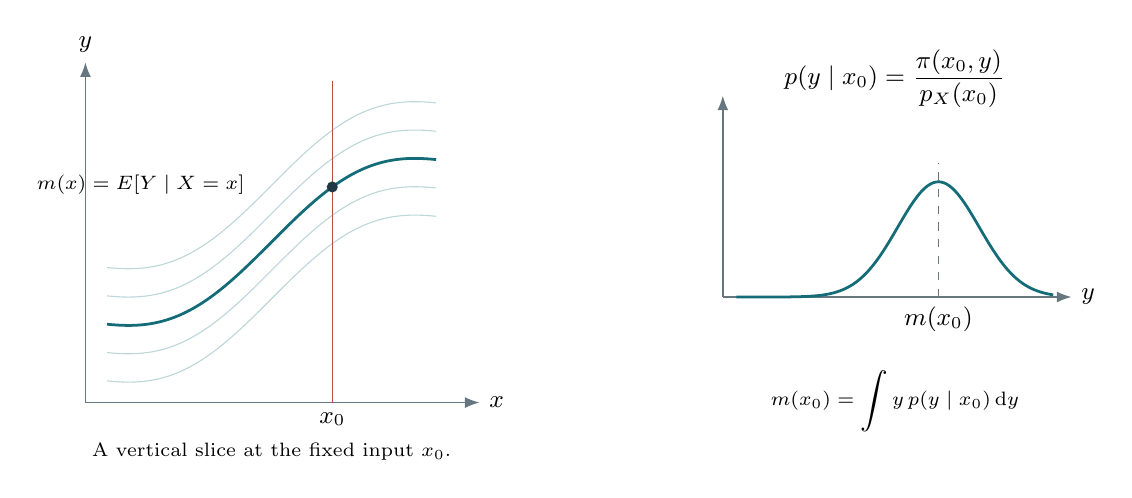
\begin{tikzpicture}[x=1cm,y=1cm]
\pgfmathsetmacro{\conditionalmean}{.28+.35*sin(59.5)}
\begin{scope}[x=1.1cm,y=1.2cm]
\draw[axis] (-2.15,-1.7)--(2.4,-1.7) node[right] {$x$};
\draw[axis] (-2.15,-1.7)--(-2.15,1.9) node[above] {$y$};
\foreach \shift in {-.6,-.3,.3,.6}{\draw[accent!28,domain=-1.9:1.9,samples=100] plot (\x,{.4*\x+.35*sin(85*\x)+\shift});}
\draw[curve,domain=-1.9:1.9,samples=100] plot (\x,{.4*\x+.35*sin(85*\x)});
\draw[signalred] (.7,-1.7)--(.7,1.7);
\fill[ink] (.7,\conditionalmean) circle(2pt);
\node[below] at (.7,-1.7) {$x_0$};
\node[above left,font=\scriptsize] at (-.2,.4) {$m(x)=\mathbb E[Y\mid X=x]$};
\node[font=\scriptsize] at (0,-2.22) {A vertical slice at the fixed input $x_0$.};
\end{scope}
\begin{scope}[shift={(7.8,-.7)},x=1.15cm,y=1.65cm]
\draw[axis] (-1.8,0)--(2.05,0) node[right] {$y$};
\draw[axis] (-1.8,0)--(-1.8,1.55);
\draw[curve,domain=-1.65:1.85,samples=160] plot (\x,{exp(-((\x-\conditionalmean)/.45)^2/2)/(.45*sqrt(2*pi))});
\draw[guide] (\conditionalmean,0)--(\conditionalmean,1.03);
\node[below] at (\conditionalmean,0) {$m(x_0)$};
\node[align=center] at (.1,1.68) {$\displaystyle p(y\mid x_0)=\frac{\pi(x_0,y)}{p_X(x_0)}$};
\node[font=\scriptsize,align=center] at (.1,-.8) {$\displaystyle m(x_0)=\int y\,p(y\mid x_0)\,\mathrm dy$};
\end{scope}
\end{tikzpicture}
\end{document}
